\documentclass[a4paper,12pt,oneside]{book}
\usepackage[T1]{fontenc}                                      
\usepackage[utf8]{inputenc}                               
\usepackage[italian]{babel}
\usepackage{amsfonts}
\usepackage{amsthm}
\usepackage{amsmath,amssymb}
\usepackage{array}
\usepackage{arydshln}
\usepackage{braket}
\usepackage{blindtext}
\usepackage{calc}
\usepackage{cancel}
\usepackage{caption}
\usepackage{epsfig}
\usepackage{eucal}
\usepackage{fancyhdr}
\usepackage{geometry}
\usepackage{graphicx}
\usepackage{indentfirst}
\usepackage{hhline}
\usepackage{hyperref}
\hypersetup{
			colorlinks=true,
			linkcolor=black,
			anchorcolor=black,
			citecolor=black,
			urlcolor=black,
			pdftitle={Appunti di Meccanica Quantistica},
			pdfauthor={Vittorio Lubicz}
}

\usepackage{latexsym}
\usepackage{listings} 
\usepackage{longtable}
\usepackage{makeidx}
\usepackage{mathrsfs}
\usepackage{mathdots}
\usepackage{multirow}
\usepackage{nicefrac}
\usepackage{pdfpages}
\usepackage{physics}
\usepackage{setspace}
\usepackage{tikz}
\usepackage{tikz-3dplot}
\usepackage{textcomp}
\usepackage{titlesec,color}
\usepackage{vmargin}
\setpapersize{A4}
\setmarginsrb{35mm}{30mm}{35mm}{30mm}%
             {0mm}{10mm}{0mm}{10mm}



\definecolor{gray75}{gray}{0.75}
\newcommand{\hsp}{\hspace{20pt}}

\titleformat{\chapter}[hang]{\huge\bfseries}{\myfont{\textit{\large{\chaptername\hspace{1pt} \thechapter\hspace{3pt}}}}\textcolor{gray75}{$\mid$}\hspace{0.4cm}}{0pt}{\myfont{\huge\bfseries}}

\titleformat{\section}[hang]{\large\bfseries}{\myfont{\textit{\normalsize{\thesection\hspace{2pt}}}}\hspace{0.4cm}}{0pt}{\myfont{\Huge\bfseries}}

\titleformat{\subsection}[hang]{\large\bfseries}{\myfont{\textit{\small{\thesubsection\hspace{2pt}}}}\hspace{0.4cm}}{0pt}{\myfont{\huge\bfseries}}

\renewcommand{\chaptermark}[1]{\markboth{#1}{}}
\renewcommand{\sectionmark}[1]{\markright{#1}}
\newcommand*{\myfont}{\fontfamily{ppl}\selectfont}

\begin{document}

%*****************LAYOUT PAGINE**************************
\fancypagestyle{plain}{%
\fancyhf{} % cancella tutti i campi di  intestazione e pi\`e di pagina
\fancyfoot[C]{\bfseries \myfont{\thepage}} % tranne il centro
\renewcommand{\headrulewidth}{0pt}
\renewcommand{\footrulewidth}{0pt}}

\fancypagestyle{VS}{
\headheight = 15pt
\lhead[\myfont{\textit{\textbf{\thechapter\nouppercase{\leftmark}}}}]{\myfont{\textit{\textbf{\nouppercase{\leftmark}}}}}
\chead[]{}
\rhead[\myfont{\textbf{\thepage}}]{\myfont{\textbf{\thepage}}}

\lfoot[]{}
\cfoot[]{}
\rfoot[]{}
}
%*******************************************************



\pagestyle{VS}

\setcounter{chapter}{6}
\setcounter{page}{78}
\chapter[Traslazioni e impulso]{Traslazioni e impulso\footnote{S1.6, LL15}}
La stretta connessione esistente in meccanica classica \textbf{tra impulso e traslazioni spaziali} vale anche nella meccanica quantistica.\\
In meccanica quantistica, così come in meccanica classica, \textbf{per un sistema che è invariante rispetto a traslazioni lungo un determinato asse, si conserva la componente dell'impulso parallela al dato asse.} Inoltre ance in meccanica quantistica è possibile affermare che \textbf{l'impulso è il generatore delle traslazioni spaziali.}\\
Per introdurre il concetto di traslazione spaziale in meccanica quantistica, consideriamo un sistema che sia ben localizzato nell'intorno di un punto $\vec{x}'$ nello spazio, e sia rappresentato pertanto dal valore di stato $\vert \vec{x}' \rangle$. Consideriamo poi una trasformazione che cambia questo stato in un altro stato ben localizzato, questa volta attorno al punto $\mathbf{\vec{x}'+ d\vec{x}'}$. Tutti gli altri parametri da cui dipende lo stato del sistema restano immutati nella trasformazione. L'operatore che realizza questa trasformazione è detto \textbf{operatore di traslazione infinitesima} di $d\vec{x}'$ e lo indichiamo con $\mathbf{T(d\vec{x}')}$. La sua azione sullo stato
 $\vert \vec{x}' \rangle$ è pertanto definito da:
\begin{equation}
T(d\vec{x}')\vert \vec{x}' \rangle=\vert \vec{x}'+ d\vec{x}' \rangle .
\end{equation}
Questa espressione definisce \textbf{l'azione dell'operatore $\mathbf{T(d\vec{x}')}$ su uno stato arbitrario $\mathbf{\vert \alpha \rangle}$}, giacché questo può essere sempre sviluppato in serie di autostati dell'operatore di posizione:
\begin{eqnarray}
T(d\vec{x}') \vert \alpha \rangle & = & T(d\vec{x}') \int d^3x' \ \vert \vec{x}' \rangle \langle \vec{x}' \vert \alpha \rangle =  \nonumber \\
& = & \int d^3x' \ \vert \vec{x}' + d \vec{x}' \rangle \langle \vec{x}' \vert \alpha \rangle 
\end{eqnarray}
ossia
\begin{equation}
T(d\vec{x}') \vert \alpha \rangle  = \int d^3x' \ \vert \vec{x}'  \rangle \langle \vec{x}' - d \vec{x}' \vert \alpha \rangle .
\end{equation}
Vediamo che la f.d.o. corrispondente allo stato traslato di $\vert \alpha \rangle $ si ottiene a partire dalla f.d.o. dello stato $\vert \alpha \rangle $ mediante la sostituzione $\vec{x}' \rightarrow \vec{x}'-d\vec{x}'$.\\
Sia il vettore di stato $vert \alpha \rangle$ che il vettore di stato $T(d\vec{x}') \vert \alpha \rangle$ devono essere normalizzati, ossia
\begin{equation}
\langle \alpha \vert \alpha \rangle = \langle \alpha \vert T^+(d\vec{x}') T(d\vec{x}') \vert \alpha \rangle .
\end{equation}
In altri termini \textbf{l'operatore di traslazione deve essere unitario:}
\begin{equation}
T^+(d\vec{x}') T(d\vec{x}') =1 .
\end{equation}
È evidente che la condizione di unitarietà deve essere soddisfatta non solo dall'operatore di traslazione infinitesima ma anche dall'operatore di traslazione finita, così come, più in generale, da un qualunque operatore che effettua trasformazioni tra vettori di stato.\\
Nel limite di $d\vec{x}' \rightarrow 0$ l'operatore $T(d\vec{x}')$ deve ridursi ovviamente all'identità. Inoltre, l'effetto combinato di due traslazioni successive di $d\vec{x}'$ e $d\vec{x}''$ rispettivamente, deve essere equivalente ad una traslazione del vettore $d\vec{x}'+d\vec{x}''$: 
\begin{equation}
T(d\vec{x}')\ T(d\vec{x}'') = T(d\vec{x}'+d\vec{x}'').
\end{equation}
Queste considerazioni ci consentono di scrivere, al primo ordine in $d\vec{x}'$:
\begin{equation}
\label{eq:cap7_1}
T(d\vec{x}')=1-i\vec{k}\cdot d\vec{x}' ,
\end{equation}
dove $\vec{k}$ è un operatore di componenti $k_x$, $k_y$ e $k_z$.\\
Il fattore $i$, introdotto nell'eq. \eqref{eq:cap7_1}, comporta che \textbf{l'operatore ${\vec{k}}$ è hermitiano}. Dalla condizione di unitarietà di $T$ segue infatti
\begin{eqnarray}
T^+(d\vec{x}') T(d\vec{x}') & = & \left(1+i\vec{k}^+\cdot d\vec{x}'\right) \left(1-i\vec{k}\cdot d\vec{x}'\right) \nonumber \\ 
& = & 1-i\left(\vec{k}-\vec{k}^+\right)\cdot d\vec{x}'+O({d\vec{x}' }^2) 
\end{eqnarray}
da cui
\begin{equation}
\vec{k}=\vec{k}^+ .
\end{equation}
L'operatore $\vec{k}$, così come definito dall'eq.\eqref{eq:cap7_1}, è detto in meccanica quantistica il \textbf{generatore delle traslazioni}.\\
Il significato fisico di $\vec{k}$ può essere derivato dalla meccanica classica. Una traslazione infinitesima in meccanica classica può essere considerata come una trasformazione canonica
\begin{equation}
\vec{X}= \vec{x}+ d\vec{x}, \quad \vec{P}= \vec{p} ,
\end{equation}
ottenibile dalla funzione generatrice
\begin{equation}
\label{eq:cap7_2}
\Phi = \vec{x}\cdot \vec{P}+\vec{P}\cdot d\vec{x} ,\qquad\left[\Phi=\Phi ( \vec{x}, \vec{P} ) \right].
\end{equation}
Poiché $\vec{x} \cdot \vec{P}$ è la funzione generatrice della trasformazione identità, riconosciamo che l'eq.\eqref{eq:cap7_2} ha una stretta somiglianza con l'operatore di traslazione infinitesimo, definito dall'eq.\eqref{eq:cap7_1}. Siamo quindi indotti a  formulare l'ipotesi che l'operatore $\vec{k}$ coincida, a meno di un fattore costante, con l'operatore impulso. La costante di proporzionalità deve avere le dimensioni dell'inverso di un'azione e risulta essere uguale all'inverso della costante di Planck, $\hbar ^{-1}$. Dunque:
\begin{equation}
\vec{k}=\frac{\vec{p}}{\hbar}.
\end{equation}
Con questa identificazione l'operatore di traslazione infinitesima si scrive
\begin{equation}
\label{eq:cap7_3}
T(d\vec{x}') = 1-\frac{1}{\hbar}\vec{p}\cdot\vec{x}.
\end{equation}
Il valore numerico della costante universale $\hbar$, che dipende peraltro dal sistema di unità di misura adottato, non può essere determinato sulla base di principi primi della teoria quantistica ma può essere solo misurato negli esperimenti. \\
È semplice derivare, a partire dall'espressione \eqref{eq:cap7_3} dell'operatore di traslazione infinitesima, la forma esplicita dell'operatore che effettua \textbf{traslazioni di una quantità finita}. Considerando ad esempio una traslazione finita di una quantità $\Delta x '$ nella direzione dell'asse $x$. Questa trasformazione può essere considerata come il prodotto di $N$ traslazioni infinitesime, di una quantità $\Delta x ' / N$, nella direzione dell'asse $x$, nel limite $N\rightarrow \infty $. Troviamo allora:
\begin{eqnarray}
T(\Delta x'\hat{x}) & = & \lim _{N\rightarrow \infty} \left(T \left( \frac{\Delta x'}{N}\hat{x} \right) \right) ^N = \lim _{N\rightarrow \infty} \left( 1- \frac{i p_x \Delta x'}{\hbar N} \right) ^N =\nonumber \\
&=& \lim _{N\rightarrow \infty} \exp \left[N\ \log \left(1- \frac{i p_x \Delta x'}{\hbar N}  \right) \right] = \nonumber \\
&=& \exp \left[  -\frac{i p_x \Delta x'}{\hbar}  \right] 
\end{eqnarray}
ossia
\begin{equation}
T(\Delta x'\hat{x}) = e^{-\frac{i}{\hbar} p_x \Delta x' }.
\end{equation}
\section[Le regole di commutazione canoniche e la relazione di indeterminazione di Heisenberg]{Le regole di commutazione canoniche e la relazione di indeterminazione di Heisenberg\footnote{S1.6, LL16}}
poniamoci in primo luogo il problema di derivare le \textbf{regole di commutazione tra le diverse componenti dell'operatore impulso}.\\
Una proprietà fondamentale delle traslazioni è che \textbf{traslazioni successive in direzioni diverse commutano}. Così, ad esempio, l'effetto combinato di una traslazione di $\Delta x'$ lungo l'asse $x$ ed una traslazione di $\Delta y'$ lungo l'asse $y$ è lo stesso di quello ottenuto da una traslazione di $\Delta y'$ lungo l'asse $y$ seguita da una traslazione di $\Delta x'$ lungo l'asse $x$:\\
\begin{figure}[!htbp]
\begin{center}
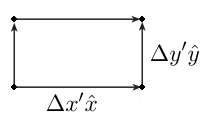
\includegraphics[scale=.8]{immagini/cap_7/fig7_1.png}
\end{center}
\end{figure}\\
Matematicamente questa circostanza si esprime come:
\begin{equation}
T(\Delta y'\hat{y})T(\Delta x'\hat{x})= T(\Delta x'\hat{x})T(\Delta y'\hat{y}),
\end{equation}
o, equivalentemente
\begin{equation}
\left[ T(\Delta x'\hat{x}), T(\Delta y'\hat{y})\right] =0.
\end{equation}
Espresso in termini dell'operatore quantità di moto, il commutatore delle due traslazioni si scrive:
\begin{eqnarray}
0 & = & \left[ T(\Delta x'\hat{x}), T(\Delta y'\hat{y})\right] =   \nonumber \\
 & = & \left[\left( 1-\frac{i p_x \Delta x'}{\hbar}-\frac{ {p_x} ^2 {\Delta x'}^2}{2\hbar ^2+\dots}\right), \left( 1-\frac{i p_y \Delta y'}{\hbar}-\frac{ {p_y} ^2 {\Delta y'}^2}{2\hbar ^2+\dots}\right) \right] = \nonumber  \\
& = & -\frac{1}{\hbar ^2}\left[p_x, p_y \right]\Delta x' \Delta y' + \dots
\end{eqnarray}
Ma per l'arbitrarietà degli spostamenti $\Delta x'$ e  $\Delta y'$ questa condizione conduce a
\begin{equation}
\left[p_x , p_y\right] =0,
\end{equation}
o, più in generale
\begin{equation}
\left[p_i , p_j\right] =0.
\end{equation}
Questo significa che \textbf{tutte e tre le componenti dell'impulso di una particella possono avere simultaneamente valori determinati}.\\
Stabiliamo le \textbf{regole di commutazione tra gli operatori impulso e gli operatori coordinate}. A tale scopo deriviamo dapprima la regola di commutazione tra l'operatore di posizione e l'operatore di traslazione infinitesima. Applicando ad un generico autoket della posizione separatamente l'operatore $\vec{x}\ T(d\vec{x}')$ o l'operatore$T(d\vec{x}')\ \vec{x}$ otteniamo:
\begin{eqnarray}
& & \vec{x}\ T(d\vec{x}')\vert \vec{x}' \rangle = \vec{x}\vert\vec{x}'+d\vec{x}'\rangle =\underbrace{\vec{x}'+d\vec{x}'}_{\textrm{autoval.}}\vert\vec{x}'+d\vec{x}'\rangle ,  \\
 \nonumber \\
& & T(d\vec{x}')\ \vec{x} \vert \vec{x}' \rangle = \underbrace{\vec{x}'}_{\textrm{autoval.}} T(d\vec{x}')\vert \vec{x}'\rangle = \vec{x}'\vert \vec{x}'+d\vec{x}'\rangle ,
\end{eqnarray}
da cui, sottraendo membro a membro
\begin{equation}
\left[\vec{x}, T(d\vec{x}')\right]\vert \vec{x}' \rangle = d\vec{x}' \vert \vec{x}' \rangle ,
\end{equation}
ma poiché uno stato arbitrario $\vert \alpha \rangle $ può essere sempre espresso come combinazione lineare di autostati della posizione, la precedente equazione vale per uno stato arbitrario e può dunque essere considerata un'identità operatoriale:
\begin{equation}
\left[\vec{x}, T(d\vec{x}')\right] = d\vec{x}'  .
\end{equation}
In termini dell'operatore impulso il commutatore si scrive
\begin{equation}
\left[ \vec{x}, 1- \frac{i}{\hbar}\vec{p}\cdot d\vec{x}'\right] =-\frac{i}{\hbar}\left(d\vec{x}'\cdot \vec{p}-\vec{p}\cdot d\vec{x}' \right) =d\vec{x}' .
\end{equation}
Consideriamo allora la componente i-esima di questa equazione e consideriamo uno spostamento $d\vec{x}'$ nella direzione dell'asse $j$. Troviamo in tal modo:
\begin{equation}
-\frac{i}{\hbar}\left( x_ip_j-p_jx_i\right) =\delta _{ij},
\end{equation}
ossia
\begin{equation}
\left[ x_i, p_j \right] =\delta _{ij}.
\end{equation}
Questa equazione dimostra che \textbf{la coordinata e la componente dell'impulso di una particella non possono essere misurate simultaneamente lungo uno stesso asse. In particolare, allora, la particella non può trovarsi in un punto determinato dello spazio e, al tempo stesso, avere una quantità di moto determinata.} D'altra parte, le precedenti relazioni di commutazione dimostrano che la coordinata della particella lungo uno degli assi può avere un valore determinato simultaneamente con le componenti dell'impulso secondo gli altri due assi.\\
La relazione di indeterminazione generale
\begin{equation}
\langle \left( \Delta A\right)^2\rangle \langle \left( \Delta B\right)^2\rangle \geq \frac{1}{4}\vert \langle \left[A,B\right] \rangle \vert ^2 ,
\end{equation}
derivata precedentemente per una coppia qualunque di operatori hermitiani $A$ e $B$, può essere applicata qui al caso gli operatori $x$ e $p_x$ per ottenere
\begin{equation}
\Delta x \cdot \Delta p_x \geq \frac{\hbar}{2} ,
\end{equation}
dove si è posto $\Delta x = \sqrt{\left(\Delta x\right) ^2}$ e $\Delta p_x = \sqrt{\left(\Delta p_x\right) ^2}$. La precedente equazione costituisce la famosa \textbf{relazione di indeterminazione di Heisenberg}, derivata da Heisenberg nel 1957.\\
L'insieme delle regole di commutazione
\begin{eqnarray}
& &\left[ x_i, x_j\right]=0 \nonumber\\
& &\left[ p_i, p_j\right]=0\\
& &\left[ x_i, p_j\right]=i\hbar \delta _{ij}\nonumber 
\end{eqnarray}
vengono dette \textbf{relazioni di commutazione canoniche} e costituiscono uno dei fondamenti della meccanica quantistica.\\
È evidente la somiglianza di queste relazioni con le relazioni
\begin{eqnarray}
& &\left\{ x_i, x_j\right\}=0 \nonumber\\
& &\left\{ p_i, p_j\right\}=0\\
& &\left\{ x_i, p_j\right\}=\delta _{ij}\nonumber 
\end{eqnarray}
valida per le \textbf{parentesi di Poisson} nella meccanica classica. Fu \textbf{Dirac} ad osservare per primo questa circostanza. Egli postulò allora che \textbf{le varie relazioni di commutazione della meccanica quantistica possono essere ottenute dalle corrispondenti relazioni classiche semplicemente sostituendo alle parentesi di Poisson i commutatori nel modo seguente:}
\begin{equation}
\left\{ \quad, \quad \right\} _{\textrm{classica}} \rightarrow \frac{i}{\hbar}\left[ \quad, \quad \right] .
\end{equation}
Questa ipotesi è consistente con il fatto che quando si passa al limite classico, l'operatore $i\left[ \quad, \quad \right]$ in prima approssimazione diventa zero.\\
È evidente tuttavia che l'assunzione di Dirac non consente comunque di stabilire, sulla base del limite classico, per quelle quantità, quali lo spin, che non hanno analogo classico.
\section[L'operatore impulso nella rappresentazione delle coordinate. Autofunzioni dell'impulso]{L'operatore impulso nella rappresentazione \\delle coordinate. Autofunzioni dell'impulso \footnote{S1.7, LL15}}
Consideriamo ora come si esprime l'operatore \textbf{impulso nella rappresentazione elle coordinate.}\\
A tale scopo esaminiamo nuovamente l'azione dell'operatore di traslazione infinitesima su un generico vettore di stato $\vert \alpha \rangle$. Riferendoci per semplicità al caso di una singola dimensione spaziale ed indicando per convenienza con $\Delta x'$ lo spostamento infinitesimo, abbiamo:
\begin{eqnarray}
\langle x' \vert T(dx') \vert \alpha \rangle 
& = & \langle x' \vert \left(1-\frac{i}{\hbar}p\ dx'\right) \vert \alpha \rangle = \langle x' \vert \left(1+\frac{i}{\hbar}p\ dx'\right) ^+ \vert \alpha \rangle = \nonumber \\
& = & \langle x'-dx'\vert \alpha \rangle = \langle x'\vert \alpha \rangle  - dx' \frac{\partial}{\partial x'} \langle x'\vert \alpha \rangle 
\end{eqnarray}
\begin{equation}
 \Rightarrow \frac{i}{\hbar}\langle x'\vert p \vert \alpha \rangle = \frac{\partial}{\partial x'}\langle x'\vert \alpha \rangle ,
\end{equation}
o anche
\begin{equation}
\label{eq:cap7_4}
\Rightarrow \langle x'\vert p \vert \alpha \rangle =-i\hbar\frac{\partial}{\partial x'}\langle x'\vert \alpha \rangle ,
\end{equation}
da cui segue anche:
\begin{equation}
\langle x'\vert p \vert x'' \rangle =-i\hbar\frac{\partial}{\partial x'}\delta (x'-x'').
\end{equation}
Dall'eq.\eqref{eq:cap7_4} possiamo derivare un'espressione esplicita per gli elementi di matrice $\langle \beta \vert p\vert \alpha \rangle $ in termini della f.d.o degli stati $\vert \beta \rangle $ ed $\vert \alpha \rangle $:
\begin{eqnarray}
\label{eq:cap7_5}
\langle \beta \vert p \vert \alpha \rangle &=& \int dx' \ \langle \beta \vert x' \rangle \left( -i\hbar \frac{\partial}{\partial x'}\right) \langle x' \vert \alpha \rangle  \nonumber \\
& = &\int dx' \ \psi _{\beta} ^* (x) \left( -i\hbar \frac{\partial}{\partial x'}\right) \psi _{\alpha}  (x') .  
\end{eqnarray}
Frequentemente si usa indicare un operatore con la sua rappresentazione nella base delle coordinate. Nel caso dell'operatore impulso questa identificazione conduce allora a
\begin{equation}
\label{eq:cap7_6}
p_x= -i\hbar \frac{\partial}{\partial x} ,
\end{equation}
o, nel caso generale di tre dimensioni
\begin{equation}
\vec{p}= -i\hbar \vec{\nabla}.
\end{equation}
Questa identificazione va intesa esattamente nel senso indicato dall'equazione \eqref{eq:cap7_5}.\\
Introduciamo ora gli \textbf{autostati dell'operatore impulso}, ossia gli stati per i quali l'impulso della particella ha un valore determinato. Continuando per semplicità a considerare il caso di una dimensione, questi stati soddisfano l'equazione
\begin{equation}
p | p' \rangle = p' | p' \rangle.
\end{equation}
Le funzioni d'onda corrispondenti agli autostati dell'impulso, ossia le ampiezze $\langle x' | p' \rangle$, sono anche dette \textbf{autofunzioni dell'operatore impulso}. L'espressione esplicita per queste autofunzioni può essere ottenuta considerando l'eq. \eqref{eq:cap7_4} nel caso in cui $| \alpha \rangle$ sia un autostato dell'impulso:
\begin{equation}
\langle x' | p | p' \rangle = -i \hbar \frac{\partial}{\partial x'} \langle x' | p' \rangle,
\end{equation}
\noindent ossia
\begin{equation}
\label{eq:cap7_7}
-i \hbar \frac{\partial}{\partial x'} \langle x' | p' \rangle = p' \langle x' | p' \rangle.
\end{equation}
Vediamo allora che, in generale, l'autostato di un operatore e la corrispondente autofunzione soddisfano la stessa equazione purché si intenda, nel secondo caso, identificare l'operatore con la sua espressione nella rappresentazione delle coordinate, come in eq. \eqref{eq:cap7_6}.\\
La soluzione dell'equazione differenziale \eqref{eq:cap7_7} per le \textbf{autofunzioni dell'operatore impulso} è
\begin{equation}
\label{eq:cap7_8}
\Psi_{p'}(x') \equiv \langle x' | p' \rangle = \mathcal{N} e^{\frac{i}{\hbar}p'x'},
\end{equation}
dove $\mathcal{N}$ è una costante di normalizzazione da determinare. Il significato fisico di questo risultato è evidente: \textbf{la probabilità che una particella che possiede un impulso determinato si trovi in una regione dello spazio compresa tra x e x+dx è una costante indipendente da x}:
\begin{equation}
\mathcal{P}(x,x+dx) = |\Psi_{p'}(x)|^2 dx = |\mathcal{N}|^2 dx.
\end{equation}
\noindent In altri termini, \textbf{in accordo con il principio di indeterminazione, una particella con impulso determinato ha un'indeterminazione totale sulla propria posizione nello spazio}.\\
L'equazione \eqref{eq:cap7_8} fornisce anche la corretta interpretazione della \emph{relazione di de Broglie}: una particella di impulso $p$ è descritta da una f.d.o. che è un'onda piana la cui lunghezza d'onda $\lambda$ è legata all'impulso $p$ dalla relazione
\begin{equation}
\lambda = \frac{2 \pi \hbar}{p} = \frac{h}{p}.
\end{equation}
Per determinare la costante di \textbf{normalizzazione delle autofunzioni dell'operatore impulso} consideriamo l'identità:
\begin{equation}
\langle x' | x'' \rangle = \int dp' \langle x' | p' \rangle \langle p' | x'' \rangle,
\end{equation}
che segue dalla relazione di completezza per gli autostati dell'impulso. Il primo membro di questa equazione è $\delta (x' - x'')$. Il secondo membro può essere calcolato utilizzando l'espressione esplicita delle autofunzioni $\langle x' | p' \rangle$ e l'espressione integrale della funzione $\delta$:
\begin{equation}
\delta (a) = \frac{1}{2 \pi} \int_{-\infty}^{+ \infty} dx ~ e^{i a x}.
\end{equation}
\noindent Si ottiene allora:
\begin{equation}
\delta (x' - x'') = |\mathcal{N}|^2 \int dp' ~ e^{\frac{i}{\hbar}p' (x' - x'')} = 2 \pi \hbar |\mathcal{N}|^2 \delta (x' - x'').
\end{equation}
Alternativamente:
\begin{eqnarray}
\langle p' | p'' \rangle &=& \int_{-\infty}^{+ \infty} dx' \langle p' | x' \rangle \langle x' | p'' \rangle = \nonumber \\
&=&  |\mathcal{N}|^2 \int_{-\infty}^{+ \infty} dx' ~ e^{-\frac{i}{\hbar}(p'-p'')x'}= \nonumber \\
&=&  |\mathcal{N}|^2 ~ 2 \pi \hbar ~ \delta (p'-p'') .
\end{eqnarray}
Scegliendo per convenzione $\mathcal{N}$ reale e positivo si ottiene allora
\begin{equation}
\Psi_{p'}(x') = \langle x' | p' \rangle = \frac{1}{\sqrt{2 \pi \hbar}} e^{\frac{i}{\hbar}p'x'}.
\end{equation}

\section[Funzioni d'onda nella rappresentazione degli impulsi]{Funzioni d'onda nella rappresentazione degli impulsi \footnote{S1.7, LL5}}
Consideriamo lo sviluppo di un generico vettore di stato $| \alpha \rangle$ in un autostato dell'operatore impulso:
\begin{equation}
| \alpha \rangle = \int dp' ~ | p' \rangle \langle p' | \alpha \rangle.
\end{equation}
I coefficienti di questo sviluppo, ossia la funzione
\begin{equation}
\Phi_\alpha (p') =  \langle p' | \alpha \rangle,
\end{equation}
determinano dunque completamente lo stato $| \alpha \rangle$.\\
La funzione $\Phi_\alpha (p')$ è detta \textbf{funzione d'onda nella rappresentazione degli impulsi}, così come la funzione
\begin{equation}
\Psi_\alpha (x') =  \langle x' | \alpha \rangle
\end{equation}
è la funzione d'onda nella rappresentazione delle coordinate.\\
Come $|\Psi_\alpha (x')|^2 dx'$ definisce la probabilità per il sistema di avere le coordinate nell'intervallo dato $dx'$, così pure $|\Phi_\alpha (p')|^2 dp'$ definisce \textbf{la probabilità che i valori dell'impulso appartengano all'intervallo dato dp'}:
\begin{equation}
\mathcal{P}(p', p'+dp') = |\langle p' | \alpha \rangle|^2 dp' = |\Phi_\alpha (p')|^2 dp'.
\end{equation}
Questa probabilità è normalizzata correttamente. Infatti, se lo stato $| \alpha \rangle$ è normalizzato, allora
\begin{eqnarray}
\langle \alpha | \alpha \rangle &=& \int_{-\infty}^{+\infty} dp' \langle \alpha | p' \rangle \langle p' | \alpha \rangle = \int_{-\infty}^{+\infty} dp' | \langle p' | \alpha \rangle |^2 = \nonumber \\
&=& \int_{-\infty}^{+\infty} dp' |\Phi_\alpha (p')|^2 = 1 .
\end{eqnarray}
\`E semplice derivare la trasformazione che lega la f.d.o. nella rappresentazione degli impulsi alla f.d.o. nella rappresentazione delle coordinate. Si ha
\begin{eqnarray}
\langle x' | \alpha \rangle &=& \int_{-\infty}^{+\infty} dp' \langle x' | p' \rangle \langle p' | \alpha \rangle =  \nonumber \\
&=& \frac{1}{\sqrt{2 \pi \hbar}} \int_{-\infty}^{+\infty} dp' ~ e^{\frac{i}{\hbar}p' \cdot x'} \langle p' | \alpha \rangle ,
\end{eqnarray}
o, equivalentemente:
\begin{equation}
\Psi_\alpha (x') = \frac{1}{\sqrt{2 \pi \hbar}} \int_{-\infty}^{+\infty} dp' ~ e^{\frac{i}{\hbar}p' \cdot x'} \Phi_\alpha (p').
\end{equation}
In modo analogo si deriva la trasformazione inversa:
\begin{equation}
\Phi_\alpha (p') = \frac{1}{\sqrt{2 \pi \hbar}} \int_{-\infty}^{+\infty} dx' ~ e^{-\frac{i}{\hbar}p' \cdot x'} \Psi_\alpha (x').
\end{equation}
Queste equazioni corrispondono matematicamente alle trasformate ed antitrasformate di Fourier.
\section[Pacchetti d'onda gaussiani]{Pacchetti d'onda gaussiani \footnote{S1.7}}
Una particella che si propaga con impulso $p$ definito è descritta, nella meccanica quantistica, da una f.d.o.:
\begin{equation}
\Psi_\alpha (x') = \langle x' | p' \rangle = \frac{1}{\sqrt{2 \pi \hbar}}~  e^{\frac{i}{\hbar}p' \cdot x'}
\end{equation}
che ha la forma di un'onda piana. La probabilità di osservare la particella in una determinata posizione è la stessa per qualunque punto dello spazio.\\
In una situazione fisica reale, tuttavia, una particella risulta sempre essere più o meno localizzata nello spazio. Questo comporta che anche il suo impulso non sia perfettamente determinato, o, equivalentemente, che lo stato della particella sia una sovrapposizione di stati con impulso definito. Le f.d.o. che descrivono tali stati vengono anche dette \textbf{pacchetti d'onda}.\\
Un esempio particolarmente importante di questo tipo è il \textbf{pacchetto d'onda gaussiano}, la cui f.d.o. nella rappresentazione delle coordinate è data da:
\begin{equation}
\Psi_\alpha (x') = \langle x' | \alpha \rangle = \frac{1}{(2 \pi \sigma^2)^{1/4}}~  e^{\frac{i}{\hbar}p_0 x' - \frac{x'^2}{4 \sigma^2}}.
\end{equation}
Per una particella che si trovi in questo stato, la distribuzione di probabilità per la coordinata $x$ è una gaussiana con valore aspettato nullo e varianza $\sigma^2$:
\begin{equation}
|\Psi_\alpha (x')|^2 = \frac{1}{\sqrt{2 \pi \sigma^2}}~   e^{- \frac{x'^2}{2 \sigma^2}}.
\end{equation}
Possiamo calcolare esplicitamente \textbf{i valori di aspettazione di x e $\mathbf x^2$}:
\begin{eqnarray}
\langle x \rangle &=& \langle \alpha | x | \alpha \rangle = \int_{-\infty}^{+\infty} dx' \langle \alpha | x | x' \rangle \langle x' | \alpha \rangle =  \nonumber \\
&=&  \int_{-\infty}^{+\infty} dx' x' \langle \alpha | x' \rangle \langle x' | \alpha \rangle = \int_{-\infty}^{+\infty} dx' x' |\Psi_\alpha (x')|^2 = 0,\\
\nonumber \\
\langle x^2 \rangle &=&  \int_{-\infty}^{+\infty} dx' x'^2 |\Psi_\alpha (x')|^2 = \frac{1}{\sqrt{2 \pi \sigma^2}} \int_{-\infty}^{+\infty} dx' x'^2 e^{- \frac{x'^2}{2 \sigma^2}} =\nonumber  \\
&=& \frac{2 \sigma^2}{\sqrt{\pi}} \int_{-\infty}^{+\infty} ds ~ s^2 ~e^{-s^2} = \frac{2 \sigma^2}{\sqrt{\pi}} ~ \Gamma(3/2) = \sigma^2,
\end{eqnarray}
ossia
\begin{equation}
\langle x \rangle = 0~~~~, ~~~~\langle x^2 \rangle = \sigma^2.
\end{equation}
Utilizzando l'espressione dell'operatore impulso nella rappresentazione delle coordinate possiamo calcolare anche \textbf{i valori di aspettazione di p e $\mathbf p^2$}. Troviamo:
\begin{eqnarray}
\langle \alpha | p | \alpha \rangle  &=&  \int_{-\infty}^{+\infty} dx' \langle \alpha | x' \rangle \left(-i \hbar \frac{\partial}{\partial x'} \right) \langle x' | \alpha \rangle = \nonumber\\
&=& \int_{-\infty}^{+\infty} dx' \Psi_\alpha(x')^* \left(-i \hbar \frac{\partial}{\partial x'} \right) \Psi_\alpha(x') = \nonumber \\
&=& \frac{1}{\sqrt{2 \pi \sigma^2}} \int_{-\infty}^{+\infty} dx' e^{-\frac{i}{\hbar}p_0 x' - \frac{x'^2}{4 \sigma^2}} \left(-i \hbar \frac{\partial}{\partial x'} \right) e^{\frac{i}{\hbar}p_0 x' - \frac{x'^2}{4 \sigma^2}} = \nonumber \\
&=& \frac{1}{\sqrt{2 \pi \sigma^2}} \int_{-\infty}^{+\infty} dx'  e^{- \frac{x'^2}{2 \sigma^2}} \left(p_0 + \frac{i \hbar}{2 \sigma^2} ~x' \right) = p_0
\end{eqnarray}
e
\begin{eqnarray}
\langle \alpha | p^2 | \alpha \rangle  &=& \int_{-\infty}^{+\infty} dx' \Psi_\alpha(x')^* \left(-i \hbar \frac{\partial}{\partial x'} \right)^2 \Psi_\alpha(x') = \nonumber \\
&=& \frac{1}{\sqrt{2 \pi \sigma^2}} \int_{-\infty}^{+\infty} dx' e^{-\frac{i}{\hbar}p_0 x' - \frac{x'^2}{4 \sigma^2}} \left(-i \hbar \frac{\partial}{\partial x'} \right)\left(p_0 + \frac{i \hbar}{2 \sigma^2} ~x' \right) e^{\frac{i}{\hbar}p_0 x' - \frac{x'^2}{4 \sigma^2}} = \nonumber \\
&=& \frac{1}{\sqrt{2 \pi \sigma^2}} \int_{-\infty}^{+\infty} dx'  e^{- \frac{x'^2}{2 \sigma^2}} \left(\frac{\hbar^2}{2 \sigma^2} + p_0^2 - \frac{\hbar^2}{4 \sigma^4}~x'^2 + \frac{i \hbar p_0}{\sigma^2}~x' \right) = \nonumber \\
&=& \frac{\hbar^2}{2 \sigma^2} + p_0^2 - \frac{\hbar^2}{4 \sigma^4} = p_0^2 + \frac{\hbar^2}{4 \sigma^4},
\end{eqnarray}
ossia:
\begin{equation}
\langle p \rangle = p_0~~~~, ~~~~\langle p^2 \rangle = p_0^2 + \frac{\hbar^2}{4 \sigma^4}.
\end{equation}
Per una particella descritta da un pacchetto d'onda gaussiano, i valori delle \textbf{dispersioni della posizione e dell'impulso} risultano:
\begin{eqnarray}
\langle (\Delta x)^2 \rangle &=& \langle x^2 \rangle - \langle x \rangle^2 = \sigma^2\\
\langle (\Delta p)^2 \rangle &=& \langle p^2 \rangle - \langle p \rangle^2 =  \frac{\hbar^2}{4 \sigma^4}.
\end{eqnarray}
Possiamo allora verificare la \textbf{relazione d'indeterminazione di Heisenberg}. In questo caso il prodotto delle indeterminazioni è dato da
\begin{equation}
\Delta x \cdot \Delta p = \frac{\hbar}{2}
\end{equation}
(dove si è posto $\Delta x \equiv \sqrt{\langle (\Delta x)^2 \rangle}$ e $\Delta p \equiv \sqrt{\langle (\Delta p)^2 \rangle}$ ) e non dipende da $\sigma$. Così \textbf{per un pacchetto d'onda gaussiano} abbiamo una relazione di uguaglianza, anziché la più generale relazione di disuguaglianza, ed \textbf{il prodotto $\mathbf{\Delta x \Delta p}$ assume il valore minimo possibile}.\\
La funzione d'onda nella rappresentazione degli impulsi per un pacchetto d'onda gaussiano è
\begin{eqnarray}
\Phi_\alpha(p') &=& \frac{1}{\sqrt{2 \pi \hbar}} \int_{-\infty}^{+\infty} dx'~ e^{-\frac{i}{\hbar} p' x'} \Psi_\alpha(x') = \\
&=& \frac{1}{\sqrt{2 \pi \hbar}} \frac{1}{(2 \pi \sigma^2)^{1/4}} \int_{-\infty}^{+\infty} dx'~ e^{-\frac{i}{\hbar} (p'-p_0) x' - \frac{x'^2}{4 \sigma^2}} = \nonumber \\
&=& \frac{1}{\sqrt{2 \pi \hbar}} \frac{1}{(2 \pi \sigma^2)^{1/4}} \int_{-\infty}^{+\infty} dx'~ e^{-\left(\frac{x'}{2 \sigma} + \frac{i}{\hbar} (p'-p_0) \sigma \right)^2 - \frac{(p'-p_0)^2}{\hbar^2}\sigma^2} = \nonumber \\
&=&  \frac{1}{\sqrt{\pi}} \left(\frac{16 \sigma^4}{4 \hbar^2 \cdot 2 \pi \sigma^2} \right)^{1/4} e^{-\frac{(p'-p_0)^2}{\hbar^2/\sigma^2}} \int_{-\infty}^{+\infty} ds ~e^{-s^2},
\end{eqnarray}
ossia
\begin{equation}
\Phi_\alpha(p') = \left(\frac{2 \sigma^2}{\pi \hbar^2} \right)^{1/4} e^{-\frac{(p'-p_0)^2}{\hbar^2/\sigma^2}}.
\end{equation}
Per un pacchetto d'onda gaussiano \textbf{la funzione d'onda nella rappresentazione degli impulsi è pure una gaussiana}. Il valore di aspettazione e la varianza di questa gaussiana sono $p_0$ e $\hbar^2/4 \sigma^2$ rispettivamente.\\
L'espressione ottenuta per la f.d.o. nella rappresentazione degli impulsi offre una via alternativa per calcolare i valori di aspettazione di $p$ e $p^2$:
\begin{eqnarray}
\langle p \rangle &=& \int_{-\infty}^{+\infty} dp' p' |\Phi_\alpha(p')|^2 = p_0\\
\langle p^2 \rangle &=& \int_{-\infty}^{+\infty} dp' p'^2 |\Phi_\alpha(p')|^2 = p_0^2 + \frac{\hbar^2}{4 \sigma^2}.
\end{eqnarray}
\section{Operatore posizione nella rappresentazione degli impulsi}
Per derivare l'espressione dell'operatore posizione nella rappresentazione degli impulsi calcoliamo esplicitamente gli elementi di matrice $\langle p' | x | p'' \rangle$. Si~ha
\begin{eqnarray}
\langle p' | x | p'' \rangle &=& \int dx' \langle p' | x | x' \rangle \langle x' | p'' \rangle = \nonumber\\
&=& \int dx' x' \langle p' | x' \rangle \langle x' | p'' \rangle = \nonumber\\
&=& \frac{1}{2 \pi \hbar} \int dx' x' e^{-\frac{i}{\hbar} (p'-p'') x'} = \nonumber \\
&=& i \hbar \frac{\partial}{\partial p'} ~\delta(p' - p'').
\end{eqnarray}
Dunque:
\begin{equation}
\langle p' | x | p'' \rangle = i \hbar~ \frac{\partial}{\partial p'} ~\delta(p' - p'').
\end{equation}
Siamo dunque in grado di esprimere, utilizzando la rappresentazione degli impulsi, l'elemento di matrice dell'operatore posizione tra due stati $| \alpha \rangle$ e $| \beta \rangle$ arbitrari:
\begin{eqnarray}
\langle \alpha | x | \beta \rangle &=& \int dp' dp'' \langle \alpha | p' \rangle \langle p' | x | p'' \rangle \langle p'' | \beta \rangle = \nonumber \\
&=& \int dp' dp'' \langle \alpha | p' \rangle \left(i \hbar \frac{\partial}{\partial p'} \right) \delta(p'-p'') \langle p'' | \beta \rangle,
\end{eqnarray}
ossia, effettuando l'integrale in $dp''$:
\begin{eqnarray}
\langle \alpha | x | \beta \rangle &=& \int dp' \langle \alpha | p' \rangle \left(i \hbar \frac{\partial}{\partial p'} \right) \langle p' | \beta \rangle = \nonumber\\
&=& \int dp'~ \Phi_\alpha(p')^* \left(i \hbar \frac{\partial}{\partial p'} \right) \Phi_\beta(p').
\end{eqnarray}
Vediamo allora che per l'operatore posizione nella rappresentazione degli impulsi vale la relazione
\begin{equation}
x = i \hbar~ \frac{\partial}{\partial p} .
\end{equation}
\end{document}